\documentclass{standalone}
\usepackage{tikz,ctex}
\usepackage{tikz-3dplot} % 2-1
\usepackage{unicode-math} % 2-5,4-1,4-2
\setmathfont{Fira Math Regular}
\setmainfont{Fira Sans}
\definecolor{background}{RGB}{239, 239, 239} % 4-5,6-2,6-5
\begin{document}
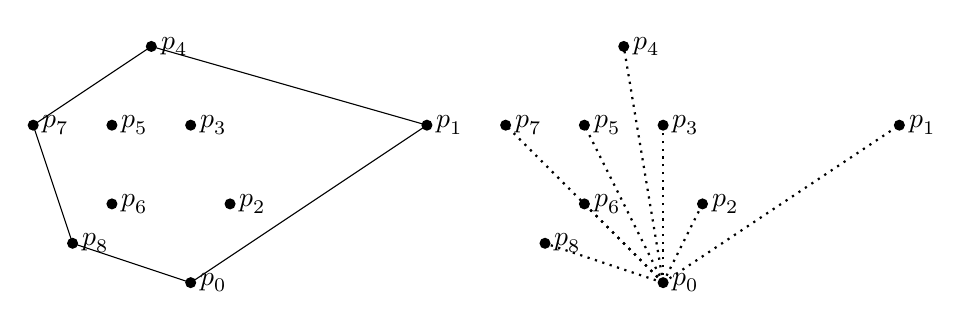
\begin{tikzpicture}
\foreach \k in{0,6}{
    \fill (0+\k,0) circle(2pt) coordinate(0\k) node[right]{$p_0$};
\foreach \x/\y[count=\i] in{3/2,.5/1,0/2,-.5/3,-1/2,-1/1,-2/2,-1.5/.5}
    \fill (\x+\k,\y) circle(2pt) coordinate(\i\k) node[right]{$p_\i$};}
\draw (00)--(10)--(40)--(70)--(80)--cycle;
\foreach \v in{16,26,...,86}
    \draw[dotted,thick] (06)--(\v);
\end{tikzpicture} 
\end{document}